\subsection{テスト関連測度}
測度は、テスト目標が達成されたかを判断するために必要である。テスト技法は道具であり、測度はその道具が目的に役立っているかを判断する根拠である。測度は、テスト計画の最適化、進捗管理、品質分析、完了判断に使われる。

\par\smallskip
\begin{center}
\centering
\IfFileExists{assets/generated_figures/ch05/fig-ch05-11.png}{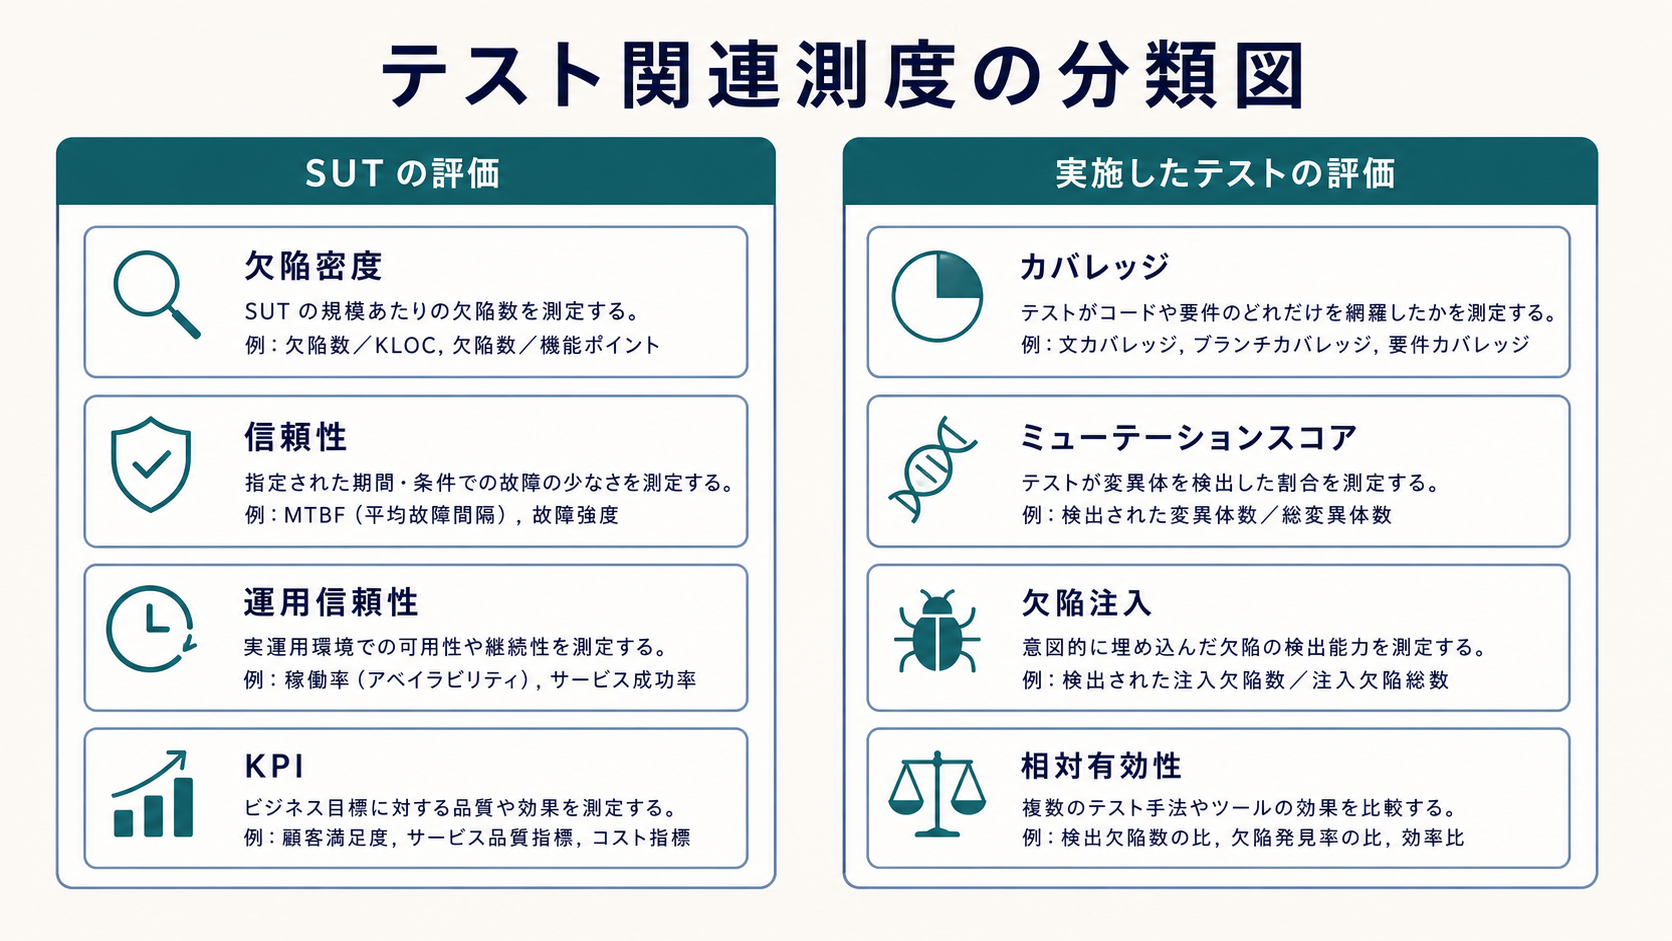
\includegraphics[width=0.96\linewidth]{assets/generated_figures/ch05/fig-ch05-11.png}}{\fbox{\parbox[c][48mm][c]{0.9\linewidth}{\centering 画像生成待ち\\テスト関連測度の分類図}}}
\par\smallskip
\refstepcounter{figure}\label{fig:ch05-11}図 \thefigure: テスト関連測度の分類図
\end{center}
図 \thefigure は、テスト関連測度の分類図を視覚的に整理したものである。
\par\smallskip

\subsubsection{SUT の評価}
SUT の評価では、テスト結果から対象システムの状態を判断する。代表的には、欠陥の種類、欠陥密度、信頼性、運用時の障害傾向、主要業績指標が使われる。

\paragraph{テスト計画と設計に役立つ SUT 測定}
テスト計画には、配備頻度、リードタイム、平均回復時間、変更失敗率などの測度が使われることがある。シフトレフトや DevOps では、これらの測度がテストの計画、管理、結果評価と強く結び付く。

\paragraph{欠陥の種類・分類・統計}
欠陥分類は、どの種類の欠陥が多いか、どの品質属性に関係するかを整理する。利用性欠陥、セキュリティ脆弱性、プライバシー攻撃、サイバーリスクなど、対象に応じて分類体系は異なる。過去の発生頻度は、どこにテスト資源を集中するかを決める根拠になる。

\paragraph{欠陥密度}
\term{欠陥密度}{Defect Density}は、見つかった欠陥数を SUT の規模で割った値である。規模にはコード行数、機能規模、モジュール数などが使われる。欠陥密度だけで品質を完全には表せないが、比較や傾向把握には役立つ。

\paragraph{寿命試験と信頼性評価}
信頼性評価は、テストをいつ止めるか、次のリリースに進めるかを判断するために使われる。クラウドやフォグ環境では、高い信頼性と可用性を維持することが重要であり、テスト活動もその評価に関わる。

\paragraph{信頼性成長モデル}
信頼性成長モデルは、観測された障害と修正の履歴から、信頼性がどのように向上するかを予測する。多くのモデルでは、障害の原因となる欠陥を修正すれば信頼性が増すと仮定する。障害数に注目するモデルと、障害間隔時間に注目するモデルがある。

\subsubsection{実施したテストの評価}
テストそのものの評価では、テストスイートがどれだけ強いか、どの技法が有効かを比較する。カバレッジ、ミューテーション分析、欠陥注入などが用いられる。

\paragraph{欠陥注入}
欠陥注入は、人工的な欠陥を SUT に入れ、テストスイートがそれらをどれだけ検出できるかを調べる。検出率からテスト有効性や残存欠陥数を推定しようとする。ただし、人工欠陥が本物の欠陥を代表しているか、挿入した欠陥を取り残さないかには注意が必要である。

\paragraph{ミューテーションスコア}
ミューテーションスコアは、殺された変異体数を生成した変異体数で割った値である。値が高いほど、テストスイートが小さな変化に敏感であることを示す。ただし、変異体の生成数が多くなるため、実行コストが問題になる。

\paragraph{技法間の比較と相対有効性}
相対有効性は、異なるテスト技法を同じ性質に対して比較する考え方である。最初の障害を見つけるまでのテスト数、欠陥検出率、信頼性改善量などが比較軸になる。
